\chapter{Approximation methods/solutions}
\begin{abox}
	Practice set 1 solutions
	\end{abox}
\begin{enumerate}
\begin{minipage}{\textwidth}
	\item If the perturbation $H^{\prime}=a x$, where $a$ is a constant, is added to the infinite square well potential
	$$
	V(x)=\left\{\begin{array}{lll}
	0 & \text { for } & 0 \leq x \leq \pi \\
	\infty & & \text { otherwise }
	\end{array}\right.
	$$
	The correction to the ground state energy, to first order in $a$, is
	\exyear{NET JUNE 2011}
\end{minipage}
\begin{tasks}(2)
	\task[\textbf{A.}] $\frac{a \pi}{2}$
	\task[\textbf{B.}]$a \pi$
	\task[\textbf{C.}]$\frac{a \pi}{4}$
	\task[\textbf{D.}]$\frac{a \pi}{\sqrt{2}}$
\end{tasks}
\begin{answer}
	$E_{0}^{1}=\int_{0}^{\pi} \psi_{0}^{*} H^{\prime} \psi_{0} d x=\frac{a \cdot 2}{\pi} \int_{0}^{\pi} x \sin ^{2} \frac{\pi x}{\pi} d x=\frac{a \pi}{2} \quad \because \psi_{0}=\sqrt{\frac{2}{\pi}} \sin \frac{\pi x}{\pi}$\\
	The correct option is \textbf{(a)}	
\end{answer}
\begin{minipage}{\textwidth}
	\item A particle in one dimension moves under the influence of a potential $V(x)=a x^{6}$, where $a$ is a real constant. For large $n$ the quantized energy level $E_{n}$ depends on $n$ as:
	\exyear{NET JUNE 2011}
\end{minipage}
\begin{tasks}(2)
	\task[\textbf{A.}] $E_{n} \sim n^{3}$
	\task[\textbf{B.}]$E_{n} \sim n^{4 / 3}$
	\task[\textbf{C.}]$E_{n} \sim n^{6 / 5}$
	\task[\textbf{D.}]$E_{n} \sim n^{3 / 2}$
\end{tasks}
\begin{answer}$\left. \right. $\\
	\begin{minipage}{0.5\textwidth}
		$V(x)=a x^{6}, H=\frac{p_{x}^{2}}{2 m}+a x^{6}, E=\frac{p_{x}^{2}}{2 m}+a x^{6}$ and $p_{x}=\left[2 m\left(E-a x^{6}\right)\right]^{\frac{1}{2}}$\\
		According to W.K.B approximation $p d x \cong n h$
		$$
		\int\left(2 m\left(E-a x^{6}\right)\right)^{1 / 2} d x \propto n
		$$
		We can find this integration without solving the integration
		$$
		E=\frac{p_{x}^{2}}{2 m}+a x^{6} \Rightarrow \frac{p_{x}^{2}}{2 m E}+\frac{x^{6}}{E / a}=1 \Rightarrow x=\left(\frac{E}{a}\right)^{\frac{1}{6}} \text { at } p_{x}=0
		$$
		Area of Ellipse $=\pi$ (semi major axis $\times$ semiminor axis)
		$$
		=\pi \sqrt{2 m E} \times\left(\frac{E}{a}\right)^{\frac{1}{6}} \propto n \Rightarrow E \propto n^{\frac{3}{2}} .
		$$
		The correct option is \textbf{(d)}
	\end{minipage}
	\begin{minipage}{0.5\textwidth}
		\begin{figure}[H]
			\centering
			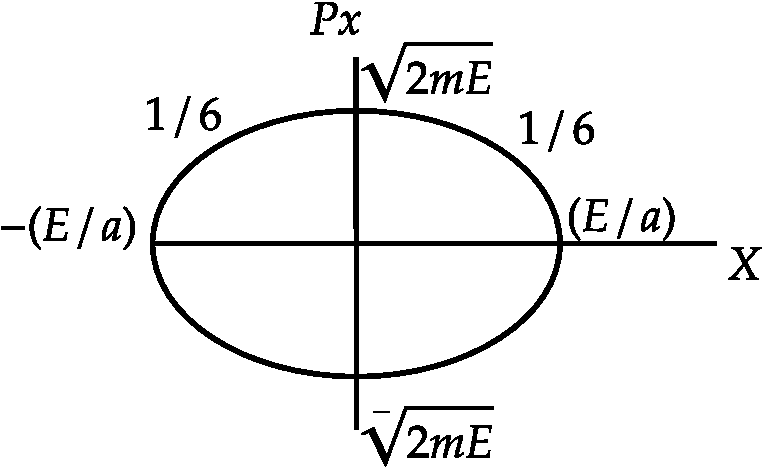
\includegraphics[height=3cm,width=5cm]{diagram-20210921-crop}
		\end{figure}
	\end{minipage}
\end{answer}
\begin{minipage}{\textwidth}
	\item The perturbation $H^{\prime}=b x^{4}$, where $b$ is a constant, is added to the one dimensional harmonic oscillator potential $V(x)=\frac{1}{2} m \omega^{2} x^{2}$. Which of the following denotes the correction to the ground state energy to first order in $b$ ?
	Hint: The normalized ground state wave function of the one dimensional harmonic oscillator potential is $\psi_{0}=\left(\frac{m \omega}{\hbar \pi}\right)^{1 / 4} e^{-m \omega x^{2} / 2 \hbar} .$ You may use the following integral $\left.\int_{-\infty}^{\infty} x^{2 n} e^{-a x^{2}} d x=a^{-n-\frac{1}{2}} \Gamma\left(n+\frac{1}{2}\right)\right]$
	\exyear{NET DEC 2011}
\end{minipage}
\begin{tasks}(2)
	\task[\textbf{A.}] $\frac{3 b \hbar^{2}}{4 m^{2} \omega^{2}}$
	\task[\textbf{B.}]$\frac{3 b \hbar^{2}}{2 m^{2} \omega^{2}}$
	\task[\textbf{C.}]$\frac{3 b \hbar^{2}}{2 \pi m^{2} \omega^{2}}$
	\task[\textbf{D.}]$\frac{15 b \hbar^{2}}{4 m^{2} \omega^{2}}$
\end{tasks}
\begin{answer}
	$H^{\prime}=b x^{4}, V(x)=\frac{1}{2} m \omega^{2} x^{2}$
	Correction in ground state is given by $E_{0}^{1}=\left\langle\psi_{0}\left|H^{\prime}\right| \psi_{0}\right\rangle$ where $\psi_{0}=\left(\frac{m \omega}{\hbar \pi}\right)^{1 / 4} e^{-\frac{m \omega x^{2}}{2 \hbar}}$.\\
	$$\begin{aligned}
	&E_{0}^{1}=\int_{-\infty}^{\infty} \psi_{0}^{*} b x^{4} \psi_{0} d x=\left(\frac{m \omega}{\hbar \pi}\right)^{\frac{1}{2}} \cdot b \int x^{4} e^{-\frac{m \omega x^{2}}{\hbar}} d x=\left(\frac{m \omega}{\hbar \pi}\right)^{\frac{1}{2}} \cdot b \int_{-\infty}^{\infty}\left(x^{2}\right)^{2} e \frac{-m \omega x^{2}}{\hbar} d x \\
	&\text { It is given in the equation } \int_{-\infty}^{\infty} x^{2 n} e^{-\alpha x^{2}} d x=\alpha^{-n-1 / 2}\left(\left(n+\frac{1}{2}\right)^{2}\right. \\
	&\text { Thus } n=2 \text { and } \alpha=\frac{m \omega}{\hbar} \\
	&\Rightarrow E_{0}^{1}=\left(\frac{m \omega}{\hbar \pi}\right)^{\frac{1}{2}} \cdot b \int_{-\infty}^{\infty}\left(x^{2}\right)^{2} e \frac{-m \omega x^{2}}{\hbar} d x=b\left(\frac{m \omega}{\hbar \pi}\right)^{\frac{1}{2}}\left(\frac{m \omega}{\hbar}\right)^{-2-\frac{1}{2}} \sqrt{\left(2+\frac{1}{2}\right)} \\
	&\Rightarrow E_{0}^{1}=b\left(\frac{m \omega}{\hbar \pi}\right)^{\frac{1}{2}}\left(\frac{m \omega}{\hbar}\right)^{\frac{-5}{2}} \sqrt{\frac{5}{2}}=\frac{3}{4} \frac{b \hbar^{2}}{m^{2} \omega^{2}} .
	\end{aligned}$$	
	The correct option is \textbf{(a)}
\end{answer}
\begin{minipage}{\textwidth}
	\item A constant perturbation as shown in the figure below acts on a particle of mass $m$ confined in an infinite potential well between 0 and $L$.\\
	\begin{figure}[H]
		\centering
		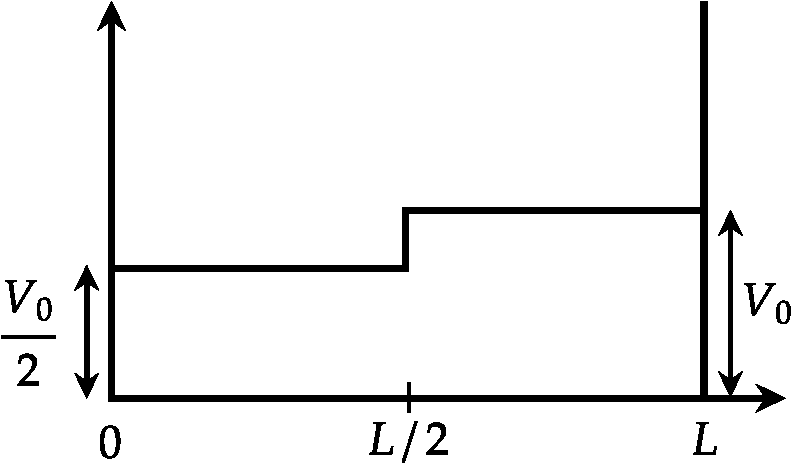
\includegraphics[height=3cm,width=5cm]{diagram-20210921(2)-crop(2)}
	\end{figure}
	$\text { The first-order correction to the ground state energy of the particle is }$
	\exyear{NET DEC 2011}
\end{minipage}
\begin{tasks}(2)
	\task[\textbf{A.}] $\frac{V_{0}}{2}$
	\task[\textbf{B.}]$\frac{3 V_{0}}{4}$
	\task[\textbf{C.}]$\frac{V_{0}}{4}$
	\task[\textbf{D.}] $\frac{3 V_{0}}{2}$
\end{tasks}
\begin{answer}
	$$\begin{aligned}
	&E_{1}^{1}=\left\langle\psi_{1}\left|V_{p}\right| \psi_{1}\right\rangle=\int_{0}^{\frac{L}{2}} \frac{V_{0}}{2} \frac{2}{L} \sin ^{2} \frac{\pi x}{L} d x+\int_{\frac{L}{2}}^{L} V_{0} \frac{2}{L} \sin ^{2} \frac{\pi x}{L} d x \\
	&E_{1}^{1}=\frac{V_{0}}{L} \int_{0}^{\frac{L}{2}} \frac{1}{2}\left(1-\cos \frac{2 \pi x}{L}\right) d x+\frac{2 V_{0}}{L} \int_{\frac{L}{2}}^{L} \frac{1}{2}\left(1-\cos \frac{2 \pi x}{L}\right) d x \\
	&\Rightarrow E_{1}^{1}=\frac{V_{0}}{2 L}\left(\frac{L}{2}\right)+\frac{2 V_{0}}{2 L}\left(L-\frac{L}{2}\right)=\frac{V_{0}}{4}+\frac{2 V_{0}}{4}=\frac{3 V_{0}}{4}
	\end{aligned}$$
	The correct option is \textbf{(b)}	
\end{answer}
\begin{minipage}{\textwidth}
	\item Consider a two-dimensional infinite square well
	$$
	V(x, y)=\left\{\begin{array}{ll}
	0, & 0<x<a, \\
	\infty, & \text { otherwise }
	\end{array} \quad 0<y<a\right.
	$$
	Its normalized Eigenfunctions are $\psi_{n_{x}, n_{y}}(x, y)=\frac{2}{a} \sin \left(\frac{n_{x} \pi x}{a}\right) \sin \left(\frac{n_{y} \pi y}{a}\right)$,
	where $n_{x}, n_{y}=1,2,3, . .$\\
	If a perturbation $H^{\prime}=\left\{\begin{array}{cc}V_{0} & 0<x<\frac{a}{2}, \quad 0<y<\frac{a}{2} \\ 0 & \text { otherwise }\end{array}\right.$ \\is applied, then the correction to the
	energy of the first excited state to order $V_{0}$ is
	\exyear{NET JUNE 2013}
\end{minipage}
\begin{tasks}(2)
	\task[\textbf{A.}] $\frac{V_{0}}{4}$
	\task[\textbf{B.}]$\frac{V_{0}}{4}\left[1 \pm \frac{64}{9 \pi^{2}}\right]$
	\task[\textbf{C.}]$\frac{V_{0}}{4}\left[1 \pm \frac{16}{9 \pi^{2}}\right]$
	\task[\textbf{D.}]$\frac{V_{0}}{4}\left[1 \pm \frac{32}{9 \pi^{2}}\right]$
\end{tasks}
\begin{answer}
	For first excited state, which is doubly degenerate
	$$
	\left|\phi_{1}\right\rangle=\frac{2}{a} \sin \frac{\pi x}{a} \sin \frac{2 \pi y}{a},\left|\phi_{2}\right\rangle=\frac{2}{a} \sin \left(\frac{2 \pi x}{a}\right) \sin \left(\frac{\pi y}{a}\right)
	$$
	$$\begin{aligned}
	&H_{11}=\left\langle\phi_{1}|H| \phi_{1}\right\rangle=V_{0} \frac{2}{a} \int_{0}^{a / 2} \sin ^{2}\left(\frac{\pi x}{a}\right) d x \frac{2}{a} \int_{0}^{a / 2} \sin ^{2}\left(\frac{2 \pi y}{a}\right) d y=V_{0} \cdot \frac{1}{2} \cdot \frac{1}{2}=\frac{V_{0}}{4} \\
	&H_{12}=\left\langle\phi_{1}|H| \phi_{2}\right\rangle \quad=V_{0} \frac{2}{a} \int_{0}^{a / 2} \sin \frac{\pi x}{a} \sin \frac{2 \pi x}{a} d x \frac{2}{a} \int_{0}^{a / 2} \sin \frac{2 \pi y}{a} \sin \frac{\pi y}{a} d y \\
	&H_{12}=V_{0}\left(\frac{4}{3 \pi}\right)\left(\frac{4}{3 \pi}\right)=V_{0} \frac{16}{9 \pi^{2}}, H_{21}=\left\langle\phi_{2}\left|H^{\prime}\right| \phi_{1}\right\rangle=V_{0} \frac{16}{9 \pi^{2}} \text { and } H_{22}=\left\langle\phi_{2}\left|H^{\prime}\right| \phi_{2}\right\rangle=\frac{V_{0}}{4} .
	\end{aligned}$$
	$$\begin{aligned}
	&\text { Thus }\left(\begin{array}{ll}
	\frac{V_{0}}{4}-\lambda & \frac{16 V_{0}}{9 \pi^{2}} \\
	\frac{16 V_{0}}{9 \pi^{2}} & \frac{V_{0}}{4}-\lambda
	\end{array}\right)=0 \Rightarrow\left(\frac{V_{0}}{4}-\lambda\right)^{2}-\left(\frac{16 V_{0}}{9 \pi^{2}}\right)^{2}=0 \\
	&\Rightarrow\left(\frac{V_{0}}{4}-\lambda\right)=\pm \frac{16 V_{0}}{9 \pi^{2}} \Rightarrow \lambda=\frac{V_{0}}{4}\left(1 \pm \frac{64}{9 \pi^{2}}\right)
	\end{aligned}$$
	The correct option is \textbf{(b)}
\end{answer}
\begin{minipage}{\textwidth}
	\item Two identical bosons of mass $m$ are placed in a one-dimensional potential $V(x)=\frac{1}{2} m \omega^{2} x^{2} .$ The bosons interact via a weak potential,
	$$
	V_{12}=V_{0} \exp \left[-m \Omega\left(x_{1}-x_{2}\right)^{2} / 4 \hbar\right]
	$$
	where $x_{1}$ and $x_{2}$ denote coordinates of the particles. Given that the ground state wavefunction of the harmonic oscillator is $\psi_{0}(x)=\left(\frac{m \omega}{\pi \hbar}\right)^{\frac{1}{4}} e^{-\frac{m \omega x^{2}}{2 \hbar}} .$ The ground state energy of the two-boson system, to the first order in $V_{0}$, is
	\exyear{NET JUNE 2013}
\end{minipage}
\begin{tasks}(2)
	\task[\textbf{A.}] $\hbar \omega+2 V_{0}$
	\task[\textbf{B.}]$\hbar \omega+\frac{V_{0} \Omega}{\omega}$
	\task[\textbf{C.}]$\hbar \omega+V_{0}\left(1+\frac{\Omega}{2 \omega}\right)^{-\frac{1}{2}}$
	\task[\textbf{D.}]$\hbar \omega+V_{0}\left(1+\frac{\omega}{\Omega}\right)$
\end{tasks}
\begin{answer}
	There are two bosons trapped in harmonic oscillator.
	So, energy for ground state without perturbation is, $2 \cdot \frac{\hbar \omega}{2}=\hbar \omega$.
	If perturbation is introduced, we have to calculate $\left\langle V_{1,2}\right\rangle$
	where $V_{1,2}=V_{0} \exp \left[-m \Omega\left(x_{1}-x_{2}\right)^{2} / 4 \hbar\right]$.
	But calculating $\left\langle V_{1,2}\right\rangle$ on state $\psi_{0}(x)=\left(\left(\frac{m \omega}{\pi \hbar}\right)^{\frac{1}{2}} e^{-\frac{m \omega x_{1}^{2}}{2 \hbar}} e^{-\frac{m \omega x_{2}^{2}}{2 \hbar}}\right)$ is very tedious task.\\
	So lets use a trick i.e perturbation is nothing but approximation used in Taylor series. So just expand $V_{1,2}=V_{0} \exp \left[-m \Omega\left(x_{1}-x_{2}\right)^{2} / 4 \hbar\right]$ and take average value of first term
	$$
	\begin{aligned}
	&V_{1,2}=V_{0} \exp \left[-m \Omega\left(x_{1}-x_{2}\right)^{2} / 4 \hbar\right]=V_{0}\left(1-\frac{m \Omega\left(x_{1}-x_{2}\right)^{2}}{4 \hbar}+\ldots\right) \\
	&=V_{0}\left(1-\frac{m \Omega\left(x_{1}^{2}+x_{2}^{2}-2 x_{1} \cdot x_{2}\right)}{4 \hbar}+\ldots\right)
	\end{aligned}
	$$
	$$\begin{aligned}
	&\left\langle V_{1,2}\right\rangle=V_{0}\left(1-\frac{m \Omega\left(\left\langle x_{1}^{2}\right\rangle+\left\langle x_{2}^{2}\right\rangle-2\left\langle x_{1}\right\rangle \cdot\left\langle x_{2}\right\rangle\right)}{4 \hbar}+\ldots\right)=V_{o}\left(1-\frac{m \Omega\left(\frac{\hbar}{2 m \omega}+\frac{\hbar}{2 m \omega}-0\right)}{4 \hbar}\right) \ldots \\
	&\Rightarrow\left\langle V_{12}\right\rangle=V_{o}\left(1-\frac{\Omega}{4 \omega}\right) \approx V_{0}\left(1+\frac{\Omega}{2 \omega}\right)^{\frac{-1}{2}}, \text { so } E=\hbar \omega+V_{0}\left(1+\frac{\Omega}{2 \omega}\right)^{\frac{-1}{2}} .
	\end{aligned}$$
	The correct option is \textbf{(c)}	
\end{answer}
\begin{minipage}{\textwidth}
	\item The bound on the ground state energy of the Hamiltonian with an attractive deltafunction potential, namely
	$$
	H=-\frac{\hbar^{2}}{2 m} \frac{d^{2}}{d x^{2}}-a \delta(x)
	$$
	using the variational principle with the trial wavefunction $\psi(x)=A \exp \left(-b x^{2}\right)$ is\\
	$\left[\text { Note }: \int_{0}^{\infty} e^{-t} t^{a} d t=\Gamma(a+1)\right]$
	\exyear{NET JUNE 2013}
\end{minipage}
\begin{tasks}(2)
	\task[\textbf{A.}] $-m a^{2} / 4 \pi \hbar^{2}$
	\task[\textbf{B.}]$-m a^{2} / 2 \pi \hbar^{2}$
	\task[\textbf{C.}]$-m a^{2} / \pi \hbar^{2}$
	\task[\textbf{D.}]$-m a^{2} / \sqrt{5} \pi \hbar^{2}$
\end{tasks}
\begin{answer}
	For given wavefunction $\langle T\rangle=\frac{\hbar^{2} b}{2 m}$ and $\langle V\rangle=-a \sqrt{\frac{2 b}{\pi}} \Rightarrow\langle E\rangle=\frac{\hbar^{2} b}{2 m}-a \sqrt{\frac{2 b}{\pi}}$\\
	For variation of parameter $\frac{d\langle E\rangle}{d b}=0 \Rightarrow \frac{d\langle E\rangle}{d b}=\frac{\hbar^{2}}{2 m}-a \sqrt{\frac{2}{\pi}} \times \frac{1}{2} b^{-1 / 2}=0 \Rightarrow b=\frac{2 m^{2} a^{2}}{\pi \hbar^{4}}$.\\ $\Rightarrow\langle E\rangle_{\min }=-\frac{m a^{2}}{\pi \hbar^{2}} .$\\
	The correct option is \textbf{(c)}
\end{answer}
\begin{minipage}{\textwidth}
	\item The ground state eigenfunction for the potential $V(x)=-\delta(x)$ where $\delta(x)$ is the delta function, is given by $\psi(x)=A e^{-\alpha|x|}$, where $A$ and $\alpha>0$ are constants. If a perturbation $H^{\prime}=b x^{2}$ is applied, the first order correction to the energy of the ground state will be
	\exyear{NET JUNE 2014}
\end{minipage}
\begin{tasks}(2)
	\task[\textbf{A.}] $\frac{b}{\sqrt{2} \alpha^{2}}$ 
	\task[\textbf{B.}]$\frac{b}{\alpha^{2}}$
	\task[\textbf{C.}]$\frac{2 b}{\alpha^{2}}$
	\task[\textbf{D.}]$\frac{b}{2 \alpha^{2}}$
\end{tasks}
\begin{answer}$\left. \right. $\\
	$\begin{aligned}
	V(x)&=-\delta(x), \psi(x)=A e^{-\alpha|x|} \\
	&\langle\psi \mid \psi\rangle=1 \Rightarrow \psi(x)=\sqrt{\alpha} e^{-\alpha|x|} \\
	&E_{1}^{1}=\left\langle\phi_{1}\left|H^{\prime}\right| \phi_{1}\right\rangle=\int_{-\infty}^{\infty} \sqrt{\alpha} e^{-\alpha|x|} b x^{2} \sqrt{\alpha} e^{-\alpha|| \mid} d x \\
	&\int_{-\infty}^{\infty} \alpha e^{-2 \alpha|x|} b x^{2} d x\\
	&=b \int_{-\infty}^{\infty} \alpha e^{-2 \alpha|x|} x^{2} d x=b \alpha\left[\int_{-\infty}^{0} x^{2} e^{2 \alpha x} d x+\int_{0}^{\infty} x^{2} e^{-2 \alpha x} d x\right]=b \alpha\left[2 \times \int_{0}^{\infty} x^{2} e^{-2 \alpha x} d x\right] \\
	&\int_{-\infty}^{\infty} \alpha e^{-2 \alpha|x|} b x^{2} d x=2 b \alpha\left[\frac{2 !}{(2 \alpha)^{3}}\right]=2 \times b \alpha \frac{2 !}{8 \alpha^{3}}=\frac{b}{2 \alpha^{2}}
	\end{aligned}$\\
	The correct option is \textbf{(d)}
\end{answer}
\begin{minipage}{\textwidth}
	\item The ground state energy of the attractive delta function potential
	$$
	V(x)=-b \delta(x) \text {, }
	$$
	where $b>0$, is calculated with the variational trial function
	$$
	\psi(x)=\left\{\begin{array}{ccc}
	A \cos \frac{\pi x}{2 a}, & \text { for } & -a<x<a, \\
	0, & & \text { otherwise, }
	\end{array}\right\} \text { is }
	$$
	\exyear{NET DEC 2014}
\end{minipage}
\begin{tasks}(2)
	\task[\textbf{A.}] $-\frac{m b^{2}}{\pi^{2} \hbar^{2}}$
	\task[\textbf{B.}]$-\frac{2 m b^{2}}{\pi^{2} \hbar^{2}}$
	\task[\textbf{C.}]$-\frac{m b^{2}}{2 \pi^{2} \hbar^{2}}$
	\task[\textbf{D.}]$-\frac{m b^{2}}{4 \pi^{2} \hbar^{2}}$
\end{tasks}
\begin{answer}
	$V(x)=-b \delta(x) ; \quad b>0 \quad \text { and } \quad \psi(x)=\left\{A \cos \frac{\pi x}{2 a} ; \quad-a<x<a\right.$\\
	$\text { Normalized } \psi=\sqrt{\frac{2}{2 a}} \cos \frac{\pi x}{2 a}$\\
	$$\begin{aligned}
	&\langle T\rangle=\int_{-a}^{a} \psi^{*}\left(\frac{-\hbar^{2}}{2 m}\right) \frac{\partial^{2}}{\partial x^{2}} \psi d x=\frac{\pi^{2} \hbar^{2}}{8 m a^{2}} \\
	&\langle V\rangle=\int_{-a}^{a} \psi^{*}-b \delta(x) \psi d x=\frac{2}{2 a}(-b)=-\frac{b}{a} \\
	&\langle E\rangle=\frac{\pi^{2} \hbar^{2}}{8 m a^{2}}-\frac{b}{a} \Rightarrow \frac{\partial\langle E\rangle}{\partial a}=\frac{-2 \pi^{2} \hbar^{2}}{8 m a^{3}}+\frac{b}{a^{2}}=0 \Rightarrow \frac{-\pi^{2} \hbar^{2}}{4 m a}+b=0 \Rightarrow a=\frac{\pi^{2} \hbar^{2}}{4 m b}
	\end{aligned}$$
	$\text { Put the value of } a \text { in equation: }\langle E\rangle=\frac{\pi^{2} \hbar^{2}}{8 m a^{2}}-\frac{b}{a}=\frac{\pi^{2} \hbar^{2}(4 m b)^{2}}{8 m\left(\pi^{2} \hbar^{2}\right)^{2}}-\frac{b(4 m b)}{\left(\pi^{2} \hbar^{2}\right)}=-\frac{2 m b^{2}}{\pi^{2} \hbar^{2}}$\\
	The correct option is \textbf{(b)}	
\end{answer}
\begin{minipage}{\textwidth}
	\item Consider a particle of mass $m$ in the potential $V(x)=a|x|, a>0$. The energy eigenvalues $E_{n}(n=0,1,2, \ldots .)$, in the WKB approximation, are
	\exyear{NET DEC 2014 }
\end{minipage}
\begin{tasks}(2)
	\task[\textbf{A.}] $\left[\frac{3 a \hbar \pi}{4 \sqrt{2 m}}\left(n+\frac{1}{2}\right)\right]^{1 / 3}$
	\task[\textbf{B.}]$\left[\frac{3 a \hbar \pi}{4 \sqrt{2 m}}\left(n+\frac{1}{2}\right)\right]^{2 / 3}$
	\task[\textbf{C.}]$\frac{3 a \hbar \pi}{4 \sqrt{2 m}}\left(n+\frac{1}{2}\right)$
	\task[\textbf{D.}]$\left[\frac{3 a \hbar \pi}{4 \sqrt{2 m}}\left(n+\frac{1}{2}\right)\right]^{4 / 3}$
\end{tasks}
\begin{answer}
	$V(x)=a|x|, \quad a>0$\\
	$\text { According to W.K.B., } \int_{\alpha_{1}}^{\alpha_{2}} p d q=\left(n+\frac{1}{2}\right) \hbar \text { where } a_{1} \text { and } a_{2} \text { are positive mid point }$\\
	$$\begin{aligned}
	&E=\frac{P^{2}}{2 m}+a|x| \Rightarrow P=\sqrt{2 m(E-a|x|)} \\
	&\int_{-E / a}^{E / a} \sqrt{2 m(E-a|x|)} d x=\left(n+\frac{1}{2}\right) \hbar \\
	&\int_{-E / a}^{0} \sqrt{2 m(E+a x)} d x+\int_{0}^{E / a} \sqrt{2 m(E-a x)} d x=\left(n+\frac{1}{2}\right) \hbar \\
	&2 \int_{0}^{E / a} \sqrt{2 m(E-a x)} d x=\left(n+\frac{1}{2}\right) \hbar
	\end{aligned}$$
	$$\begin{aligned}
	&2 m(E-a x)=t, \quad \text { At } x=0, \quad t=2 m E ; \quad x=E / a, t=0 \\
	&\Rightarrow-2 m a d x=d t \\
	&\Rightarrow 2 m a \int_{0}^{2 m E} t^{1 / 2} d t=\left.\left(n+\frac{1}{2}\right) \hbar \Rightarrow 2 m a \frac{2}{3} t^{3 / 2}\right|_{0} ^{2 m E}=\left(n+\frac{1}{2}\right) \hbar \\
	&\left.\Rightarrow \frac{4}{3} m a t^{3 / 2}\right|_{0} ^{2 m E}=\left(n+\frac{1}{2}\right) \hbar \Rightarrow \frac{4}{3} m a(2 m E)^{3 / 2}=\left(n+\frac{1}{2}\right) \hbar \\
	&\Rightarrow \frac{4}{3} \cdot 2^{3 / 2} a m^{5 / 2} E^{3 / 2}=\left(n+\frac{1}{2}\right) \hbar \Rightarrow E=\left[\frac{3 a \hbar \pi}{4 \sqrt{2 m}}\left(n+\frac{1}{2}\right)\right]^{2 / 3}
	\end{aligned}$$
	The correct option is \textbf{(b)}
\end{answer}
\begin{minipage}{\textwidth}
	\item The Hamiltonian $H_{0}$ for a three-state quantum system is given by the matrix $H_{0}=\left(\begin{array}{lll}1 & 0 & 0 \\ 0 & 2 & 0 \\ 0 & 0 & 2\end{array}\right) .$ When perturbed by $H^{\prime}=\in\left(\begin{array}{lll}0 & 1 & 0 \\ 1 & 0 & 1 \\ 0 & 1 & 0\end{array}\right)$ where $\in<<1$, the resulting shift in the energy eigenvalue $E_{0}=2$ is
	\exyear{NET DEC 2014}
\end{minipage}
\begin{tasks}(2)
	\task[\textbf{A.}] $\in,-2 \in$
	\task[\textbf{B.}] $-\in, 2 \in$
	\task[\textbf{C.}]$\pm \in$
	\task[\textbf{D.}]$\pm 2 \in$
\end{tasks}
\begin{answer}
	$H_{0}=\left(\begin{array}{lll}
	1 & 0 & 0 \\
	0 & 2 & 0 \\
	0 & 0 & 2
	\end{array}\right), \quad H^{\prime}=\epsilon_{0}\left(\begin{array}{lll}
	0 & 1 & 0 \\
	1 & 0 & 1 \\
	0 & 1 & 0
	\end{array}\right)$\\
	$\left(\begin{array}{ll}2 & 0 \\ 0 & 2\end{array}\right)$ in $H_{0}$ is not $\in_{0}\left(\begin{array}{ll}0 & 1 \\ 1 & 0\end{array}\right)$ in $H^{\prime}$ because $H^{\prime}$ is not in block diagonal form. So we must diagonalised whole $H^{\prime}$.\\ The Eigen value at $H^{\prime}=0,+\sqrt{2} \in_{0},-\sqrt{2} \in_{0}$.\\
	So $\pm \sqrt{2} \in_{0}$ is the correction for eigenvalue of $H_{0}=2$\\
	Hence none of the options given is correct.	
\end{answer}
\begin{minipage}{\textwidth}
	\item A particle of mass $m$ is in a potential $V=\frac{1}{2} m \omega^{2} x^{2}$, where $\omega$ is a constant. Let $\hat{a}=\sqrt{\frac{m \omega}{2 \hbar}}\left(\hat{x}+\frac{i \hat{p}}{m \omega}\right) .$ In the Heisenberg picture $\frac{d \hat{a}}{d t}$ is given by
	\exyear{NET JUNE 2015}
\end{minipage}
\begin{tasks}(2)
	\task[\textbf{A.}] $\omega \hat{a}$
	\task[\textbf{B.}]$-i \omega \hat{a}$
	\task[\textbf{C.}]$\omega \hat{a}^{\dagger}$
	\task[\textbf{D.}]$i \omega \hat{a}^{\dagger}$
\end{tasks}
\begin{answer}
	$V=\frac{1}{2} m \omega^{2} x^{2}$\\
	$$\begin{aligned}
	&\hat{a}=\sqrt{\frac{m \omega}{2 \hbar}}\left(\hat{x}+\frac{i \hat{p}}{m \omega}\right) \\
	&\frac{d \hat{a}}{d t}=\frac{1}{i \hbar}\langle[a, H]\rangle+\left\langle\frac{\partial a}{\partial t}\right\rangle, \quad \frac{\partial a}{\partial t}=0 \\
	&\frac{d \hat{a}}{d t}=\frac{1}{i \hbar} \sqrt{\frac{m \omega}{2 \hbar}}\left[\left[x, \frac{p^{2}}{2 m}\right]+\frac{i m \omega^{2}}{2 m \omega}\left[\hat{p}, x^{2}\right]\right]=\frac{1}{i \hbar} \sqrt{\frac{m \omega}{2 \hbar}}\left(i \hbar \frac{2 p}{2 m}+\frac{i \omega}{2}(-2 x) i \hbar\right) \\
	&=\sqrt{\frac{m \omega}{2 \hbar}}\left(\frac{p}{m}-i \omega x\right)=-i \omega \sqrt{\frac{m \omega}{2 \hbar}}\left(x+\frac{i p}{m \omega}\right)=-i \omega \hat{a}
	\end{aligned}$$
	The correct option is \textbf{(b)}
\end{answer}
\begin{minipage}{\textwidth}
	\item A hydrogen atom is subjected to the perturbation
	$$
	V_{\text {pert }}(r)=\epsilon \cos \frac{2 r}{a_{0}}
	$$
	where $a_{0}$ is the Bohr radius. The change in the ground state energy to first order in $\in$
	\exyear{NET DEC 2015}
\end{minipage}
\begin{tasks}(2)
	\task[\textbf{A.}] $\frac{\in}{4}$
	\task[\textbf{B.}] $\frac{\in}{2}$
	\task[\textbf{C.}]$\frac{-\epsilon}{2}$
	\task[\textbf{D.}] $\frac{-\epsilon}{4}$
\end{tasks}
\begin{answer}
	For First order perturbation\\
	$$\begin{aligned}
	&E_{1}^{1}=\left\langle\phi_{100}\left|V_{p}\right| \phi_{100}\right\rangle, \phi_{100}=\frac{1}{\sqrt{\pi a_{0}^{3}}} e^{\frac{-r}{a}}, V_{p}=\in \cos \left(\frac{2 r}{a_{0}}\right) \\
	&E_{1}^{1}=\int_{0}^{\infty} \frac{1}{\pi a_{0}^{3}} e^{\frac{-2 r}{a_{0}}} \in \cos \left(\frac{2 r}{a_{0}}\right) 4 \pi r^{2} d r=\frac{4 \in}{a_{0}^{3}} \int_{0}^{\infty} e^{\frac{-2 r}{a_{0}}} \cos \left(\frac{2 r}{a_{0}}\right) r^{2} d r
	\end{aligned}$$
	$$\begin{aligned}
	&=\frac{4 \in}{a_{0}^{3}} \int_{0}^{\infty} e^{\frac{-2 r}{a_{0}}}\left[\frac{e^{\frac{i 2 r}{a_{0}}}+e^{\frac{-i 2 r}{a_{0}}}}{2}\right] r^{2} d r=\frac{2 \in}{a_{0}^{3}}\left[\int_{0}^{\infty} e^{\frac{-2 r}{a_{0}}(1-i)} r^{2} d r+\int_{0}^{\infty} e^{\frac{-2 r}{a_{0}}(1+i)} r^{2} d r\right] \\
	&\Rightarrow \quad \frac{2 \in}{a_{0}^{3}}\left[\frac{2 !}{\left[\frac{2}{a_{0}}(1-i)\right]^{3}}+\frac{2 !}{\left[\frac{2}{a_{0}}(1+i)\right]^{3}}\right] \Rightarrow \frac{\epsilon}{2}\left[\frac{1}{(1-i)^{3}}+\frac{1}{(1+i)^{3}}\right]
	\end{aligned}$$
	$$\begin{aligned}
	&\Rightarrow \quad \frac{\in}{2}\left[\frac{1}{(\sqrt{2})^{3}\left(\frac{1-i}{\sqrt{2}}\right)^{3}}+\frac{1}{(\sqrt{2})^{3}\left(\frac{1+i}{\sqrt{2}}\right)^{3}}\right] \Rightarrow \frac{\epsilon}{4 \sqrt{2}}\left[\frac{1}{\left.e^{\frac{-i 3 \pi}{4}}+\frac{1}{e^{\frac{i 3 \pi}{4}}}\right]}\right. \\
	&\Rightarrow \quad \frac{\in}{4 \sqrt{2}}\left[e^{\frac{i 3 \pi}{4}}+e^{\frac{-i 3 \pi}{4}}\right] \Rightarrow \frac{\epsilon}{4 \sqrt{2}}\left[2 \cos \left(\frac{3 \pi}{4}\right)\right] \\
	&\Rightarrow \quad \frac{\in}{4 \sqrt{2}}\left[2\left(-\frac{1}{\sqrt{2}}\right)\right] \Rightarrow \frac{-\epsilon}{4} \Rightarrow E_{1}^{1}=\frac{-\epsilon}{4}
	\end{aligned}$$
	The correct option is \textbf{(d)}
\end{answer}
\begin{minipage}{\textwidth}
	\item Consider a particle of mass $m$ in a potential $V(x)=\frac{1}{2} m \omega^{2} x^{2}+g \cos k x .$ The change in the ground state energy, compared to the simple harmonic potential $\frac{1}{2} m \omega^{2} x^{2}$, to first order in $g$ is
	\exyear{NET JUNE 2016}
\end{minipage}
\begin{tasks}(2)
	\task[\textbf{A.}] $g \exp \left(-\frac{k^{2} \hbar}{2 m \omega}\right)$
	\task[\textbf{B.}]$g \exp \left(\frac{k^{2} \hbar}{2 m \omega}\right)$
	\task[\textbf{C.}]$g \exp \left(-\frac{2 k^{2} \hbar}{m \omega}\right)$
	\task[\textbf{D.}] $g \exp \left(-\frac{k^{2} \hbar}{4 m \omega}\right)$
\end{tasks}
\begin{answer}
	Ground state wavefunction
	$$
	\psi_{0}(x)=\left(\frac{m \omega}{\pi \hbar}\right)^{\frac{1}{4}} e^{-\frac{m \omega x^{2}}{2 \hbar}}
	$$
	The perturbation term is $H_{p}=g \cos k x$
	First order correction $E_{0}^{1}=\int_{-\infty}^{\infty} \psi_{0}^{*}(x) H_{P} \psi_{0}(x) d x$\\
	$$\begin{aligned}
	&=\left(\frac{m \omega}{\pi \hbar}\right)^{\frac{1}{2}} g \int_{-\infty}^{\infty} e^{-\frac{m \omega x^{2}}{\hbar}}\left(\frac{e^{i k x}+e^{-i k x}}{2}\right) d x=\frac{g}{2}\left(\frac{m \omega}{\pi \hbar}\right)^{\frac{1}{2}}\left[\int_{-\infty}^{\infty} e^{\frac{-m \omega x^{2}}{\hbar}} \cdot e^{i k x} d x+\int_{-\infty}^{\infty} e^{\frac{-m \omega x^{2}}{\hbar}} \cdot e^{-i k x} d x\right] \\
	&=\frac{g}{2}\left(\frac{m \omega}{\pi \hbar}\right)^{\frac{1}{2}} \int_{-\infty}^{\infty} e^{-\frac{m \omega x^{2}}{\hbar}+i k x} d x+\frac{g}{2}\left(\frac{m \omega}{\pi \hbar}\right)^{\frac{1}{2}} \int_{-\infty}^{\infty} e^{\frac{-m \omega x^{2}}{\hbar}-i k x} d x
	\end{aligned}$$
	From $1^{\text {st }}$ term, we have
	$$
	=\frac{g}{2}\left(\frac{m \omega}{\pi \hbar}\right)^{\frac{1}{2}} \int_{-\infty}^{\infty} e^{-\frac{m \omega}{\hbar}\left[x^{2}+\frac{2 i k \hbar}{2 m \omega}+\left(\frac{i k \hbar}{2 m \omega}\right)^{2}-\left(\frac{i k \hbar}{2 m \omega}\right)^{2}\right]} d x=\frac{g}{2}\left(\frac{m \omega}{\pi \hbar}\right)^{\frac{1}{2}} \int_{-\infty}^{\infty} e^{-\frac{m \omega}{\hbar}\left(x+\frac{i k \hbar}{2 m \omega}\right)^{2}} e^{-\frac{k^{2} \hbar}{4 m \omega}} d x
	$$
	$$
	=\frac{g}{2} e^{-\frac{k^{2} \hbar}{4 m \omega}}\left(\frac{m \omega}{\pi \hbar}\right)^{\frac{1}{2}} \int_{-\infty}^{\infty} e^{\frac{m \omega}{\hbar}\left(x+\frac{i k \hbar}{2 m \omega}\right)^{2}} d x=e^{-\frac{k^{2} \hbar}{4 m \omega}}
	$$
	Similarly, from term (ii), $\frac{g}{2}\left(\frac{m \omega}{\pi \hbar}\right)^{\frac{1}{2}} \int_{-\infty}^{\infty} e^{-\frac{m \omega x^{2}}{\hbar}-i k x} d x$
	$$
	=\frac{g}{2} e^{-\frac{k^{2} h}{4 m \omega}}\left(\frac{m \omega}{\pi \hbar}\right)^{\frac{1}{2}} \int_{-\infty}^{\infty} e^{-\frac{m \omega}{\hbar}\left(x-\frac{i k \hbar}{2 m \omega}\right)^{2}} d x=e^{-\frac{k^{2} \hbar}{4 m \omega}}
	$$
	$$
	\text { Hence, } E_{0}^{1}=\frac{g}{2}\left[e^{-\frac{k^{2} \hbar}{4 m \omega}}+e^{-\frac{k^{2} \hbar}{4 m \omega}}\right]=g e^{-\frac{k^{2} \hbar}{4 m \omega}}
	$$
	The correct option is \textbf{(d)}
\end{answer}
\begin{minipage}{\textwidth}
	\item The energy levels for a particle of mass $m$ in the potential $V(x)=\alpha|x|$, determined in the $W K B$ approximation
	$$
	\sqrt{2 m} \int_{a}^{b} \sqrt{E-V(x)} d x=\left(n+\frac{1}{2}\right) \hbar \pi
	$$
	(where $a, b$ are the turning points and $n=0,1,2 \ldots$ ), are
	\exyear{NET JUNE 2016}
\end{minipage}
\begin{tasks}(2)
	\task[\textbf{A.}] $E_{n}=\left[\frac{h \pi \alpha}{4 \sqrt{m}}\left(n+\frac{1}{2}\right)\right]^{\frac{2}{3}}$
	\task[\textbf{B.}]$E_{n}=\left[\frac{3 h \pi \alpha}{4 \sqrt{2 m}}\left(n+\frac{1}{2}\right)\right]^{\frac{2}{3}}$
	\task[\textbf{C.}]$E_{n}=\left[\frac{3 h \pi \alpha}{4 \sqrt{m}}\left(n+\frac{1}{2}\right)\right]^{\frac{2}{3}}$
	\task[\textbf{D.}] $E_{n}=\left[\frac{h \pi \alpha}{4 \sqrt{2 m}}\left(n+\frac{1}{2}\right)\right]^{\frac{2}{3}}$
\end{tasks}
\begin{answer}$\left. \right. $\\
	$\begin{aligned}
	&V(x)=\alpha|x| \\
	&\Rightarrow V(x)= \begin{cases}-\alpha x, & x<0 \\
	=\alpha x, & x>0\end{cases}
	\end{aligned}$
	$$\sqrt{2 m} \int_{a}^{b} \sqrt{E-V(x)} d x=\left(n+\frac{1}{2}\right) \pi \hbar$$
	\begin{figure}[H]
		\centering
		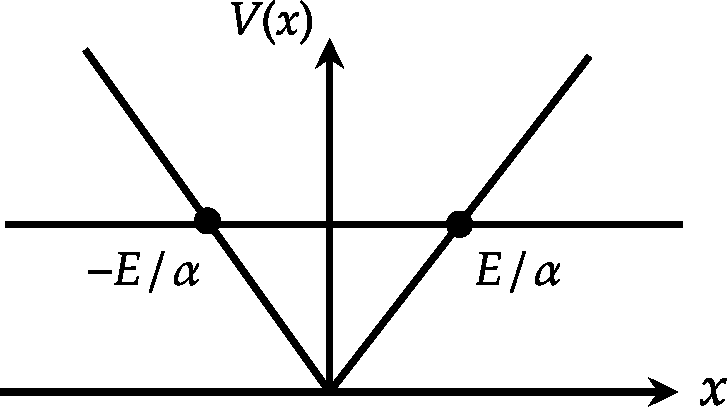
\includegraphics[height=3cm,width=5cm]{diagram-20210923(2)-crop}
		\caption{}
		\label{}
	\end{figure}
	$$\text { From figure, } a=\left(-\frac{E}{\alpha}\right), b=\left(\frac{E}{\alpha}\right) \Rightarrow \sqrt{2 m} \int_{-\frac{E}{\alpha}}^{\frac{E}{\alpha}} \sqrt{E-V(x)} d x=\left(n+\frac{1}{2}\right) \pi \hbar$$
	$\Rightarrow \sqrt{2 m} \int_{-\frac{E}{\alpha}}^{0} \sqrt{E+\alpha x} d x+\int_{0}^{\frac{E}{\alpha}} \sqrt{E-\alpha x} d x=\left(n+\frac{1}{2}\right) \pi \hbar \Rightarrow 2 \sqrt{2 m} \int_{0}^{\frac{E}{\alpha}} \sqrt{E-\alpha x}(d x)=\left(n+\frac{1}{2}\right) \pi \hbar$\\
	put $E-\alpha x=t, \quad d x=-\frac{d t}{\alpha}$\\
	$\operatorname{limit} x \rightarrow 0 \Rightarrow t \rightarrow E$\\
	$x \rightarrow \frac{E}{\alpha} \Rightarrow t \rightarrow 0$\\
	$$\begin{aligned}
	&2 \sqrt{2 m} \int_{E}^{0} \sqrt{t}\left(\frac{-d t}{\alpha}\right)=\left(n+\frac{1}{2}\right) \pi \hbar \\
	&\Rightarrow-\frac{2 \sqrt{2 m}}{\alpha}\left[\frac{2}{3} t^{\frac{3}{2}}\right]_{E}^{0}=\left(n+\frac{1}{2}\right) \pi \hbar \Rightarrow \frac{2 \sqrt{2 m}}{\alpha} \frac{2}{3} \cdot E^{\frac{3}{2}}=\left(n+\frac{1}{2}\right) \pi h \\
	&\Rightarrow E^{\frac{3}{2}}=\left(n+\frac{1}{2}\right) \frac{3 \pi \hbar \alpha}{4 \sqrt{2 m}} \Rightarrow E_{n}=\left[\frac{3 \hbar \pi \alpha}{4 \sqrt{2 m}}\left(n+\frac{1}{2}\right)\right]^{\frac{2}{3}}
	\end{aligned}$$
	The correct option is \textbf{(b)}
\end{answer}
\begin{minipage}{\textwidth}
	\item A particle of charge $q$ in one dimension is in a simple harmonic potential with angular frequency $\omega$. It is subjected to a time- dependent electric field $E(t)=A e^{-\left(\frac{t}{\tau}\right)^{2}}$, where $A$ and $\tau$ are positive constants and $\omega \tau \gg 1$. If in the distant past $t \rightarrow-\infty$ the particle was in its ground state, the probability that it will be in the first excited state as $t \rightarrow+\infty$ is proportional to
	\exyear{NET DEC 2016}
\end{minipage}
\begin{tasks}(2)
	\task[\textbf{A.}] $e^{-\frac{1}{2}(\omega \tau)^{2}}$
	\task[\textbf{B.}]$e^{\frac{1}{2}(\omega \tau)^{2}}$
	\task[\textbf{C.}] 0
	\task[\textbf{D.}]$\frac{1}{(\omega \tau)^{2}}$
\end{tasks}
\begin{answer}
	$\text { Transition probability is proportional to } P_{\text {if }} \propto\left|\int_{-\infty}^{\infty} e^{-\frac{t^{2}}{\tau^{2}}} e^{i \omega_{f i} t}\right|^{2} \text { where }$
	$$\begin{aligned}
	&\omega_{f i}=\frac{\frac{3}{2} \hbar \omega-\frac{1}{2} \hbar \omega}{\hbar}=\omega \\
	&P_{i f}=\left|\int_{-\infty}^{\infty} \exp -\frac{t^{2}}{\tau^{2}}+i \omega t d t\right|^{2}
	\end{aligned}$$
	$$\begin{aligned}
	&\text { Now calculate } \int_{-\infty}^{\infty} \exp \left(-\frac{t^{2}}{\tau^{2}}+i \omega t\right) d t=\int_{-\infty}^{\infty} \exp -\frac{1}{\tau^{2}}\left(t^{2}-i \omega t \tau^{2}+\left(\frac{i \omega \tau^{2}}{2}\right)^{2}-\left(\frac{i \omega \tau^{2}}{2}\right)^{2}\right) \\
	&=\exp \left(-\frac{\omega^{2} \tau^{2}}{4}\right) \int_{-\infty}^{\infty} \exp \frac{1}{\tau^{2}}\left(t-\frac{i \omega t}{2}\right)^{2} d t \\
	&P_{\text {if }}=\left.\left|\int_{-\infty}^{\infty} \exp -\frac{t^{2}}{\tau^{2}}+i \omega t d t\right|^{2}\right|^{2} \\
	&P_{\text {if }}=\left|\exp \left(-\frac{\omega^{2} \tau^{2}}{4}\right) \int_{-\infty}^{\infty} \exp \frac{1}{\tau^{2}}\left(t-\frac{i \omega t}{2}\right)^{2} d t\right|^{2} \\
	&P_{\text {if }} \propto \exp -\frac{\omega^{2} \tau^{2}}{2}
	\end{aligned}$$
	The correct option is \textbf{(a)}
\end{answer}
\begin{minipage}{\textwidth}
	\item A constant perturbation $H^{\prime}$ is applied to a system for time $\Delta t$ (where $H^{\prime} \Delta t<<\hbar$ ) leading to a transition from a state with energy $E_{i}$ to another with energy $E_{f}$. If the time of application is doubled, the probability of transition will be
	\exyear{NET JUNE 2017}
\end{minipage}
\begin{tasks}(2)
	\task[\textbf{A.}] unchanged
	\task[\textbf{B.}]doubled
	\task[\textbf{C.}]quadrupled
	\task[\textbf{D.}]halved
\end{tasks}
\begin{answer}
	For constant potential transition probability\\
	\begin{align*}
	&p_{i f}=4 \frac{\left|\left\langle\psi_{f}|v| \psi_{i}\right\rangle\right|^{2}}{h^{2} \omega_{f i}^{2}}\left(\sin ^{2} \frac{\omega_{f i} t_{i}}{2}\right) \\
	&\text { at } t_{i}=2 t_{i},
	\end{align*}
	\begin{align*}
	&p_{\text {if }}=\frac{4\left|\left\langle\psi_{f}|v| \psi_{i}\right\rangle\right|^{2}}{h^{2} \omega_{f i}^{2}} \sin ^{2} \frac{\omega_{f i} t_{i}}{2} \\
	&\text { at } t_{i}=2 t_{i},
	\end{align*}
	\begin{align*}
	&p_{f f}=\frac{4\left|\left\langle\psi_{f}|v| \psi_{i}\right\rangle\right|^{2}}{h^{2} \omega_{f i}^{2}} \sin ^{2}\left(\frac{\omega_{f i} 2 t_{i}}{2}\right)=\frac{4\left|\left\langle\psi_{f}|v| \psi_{i}\right\rangle\right|^{2}}{h^{2} \omega_{f i}^{2}} \sin \left(\omega_{f i} t_{i}\right) \\
	&\frac{p_{i f}}{p_{f f}}=\frac{\sin ^{2}\left(\omega_{f i} t_{i}\right)}{\sin ^{2}\left(\frac{\omega_{f i} t_{i}}{2}\right)} \Rightarrow \frac{\frac{\sin ^{2}\left(\omega_{f i} t_{i}\right)}{\omega_{f i}^{2} t_{i}^{2}} \omega_{f i}^{2} t_{i}^{2}}{\sin ^{2}\left(\frac{\omega_{f i} t_{i}}{2}\right)\left(\frac{\omega_{f i} t_{i}}{2}\right)^{2}} \quad t_{1} \rightarrow 0 \\
	&\frac{\omega_{f i}^{2} t_{i}^{2}}{2}
	\end{align*}
	\begin{align*}
	&=\frac{4 \omega_{f i}^{2} t_{i}^{2}}{\omega_{f i}^{2} t_{i}^{2}}=4 \\
	&\frac{p_{i f(2)}}{p_{i f(1)}}=4 \Rightarrow p_{i f(2)}=4 p_{i f(1)}
	\end{align*}
\end{answer}
\begin{minipage}{\textwidth}
	\item The Coulomb potential $V(r)=-e^{2} / r$ of a hydrogen atom is perturbed by adding $H^{\prime}=b x^{2}$ (where $b$ is a constant) to the Hamiltonian. The first order correction to the ground state energy is
	(The ground state wavefunction is $\psi_{0}=\frac{1}{\sqrt{\pi a_{0}^{3}}} e^{-r / a_{0}}$ )
	\exyear{NET JUNE 2017}
\end{minipage}
\begin{tasks}(2)
	\task[\textbf{A.}] $2 b a_{0}^{2}$
	\task[\textbf{B.}]$b a_{0}^{2}$
	\task[\textbf{C.}]$b a_{0}^{2} / 2$
	\task[\textbf{D.}]$\sqrt{2} b a_{0}^{2}$
\end{tasks}
\begin{answer}
	$H^{\prime}=b x^{2} \quad \text { put } x=r \sin \theta \cos \phi$\\
	\begin{align*}
	&H^{\prime}=b r^{2} \sin ^{2} \theta \cos ^{2} \phi . \\
	&E_{1}^{1}=\left\langle\psi_{1}\left|H^{\prime}\right| \psi_{1}\right\rangle,\left|\psi_{1}\right\rangle=\frac{1}{\sqrt{\pi a_{0}^{3}}} e^{-r / a_{0}} \\
	&=\int \psi_{1}^{*} H^{\prime} \psi_{1} r^{2} \sin \theta d r d \theta d \phi \\
	&=\frac{b}{\pi a_{0}^{3}} \int_{0}^{\infty} r^{2} e^{-\frac{2 r}{a_{0}}} r^{2} d r \int_{0}^{\pi} \sin ^{3} \theta d \theta \int_{0}^{2 \pi} \cos ^{2} \phi d \phi=b a_{0}^{2}
	\end{align*}
	The correct option is \textbf{(b)}
\end{answer}
\begin{minipage}{\textwidth}
	\item Consider a one-dimensional infinite square well
	$$
	V(x)=\left\{\begin{array}{lll}
	0 & \text { for } & 0<x<a \\
	\infty & & \text { otherwise }
	\end{array}\right.
	$$
	If a perturbation
	$$
	\Delta V(x)=\left\{\begin{array}{lc}
	V_{0} & \text { for } 0<x<a / 3 \\
	0 & \text { otherwise }
	\end{array}\right.
	$$
	is applied, then the correction to the energy of the first excited state, to first order in $\Delta V$, is nearest to
	\exyear{NET DEC 2017}
\end{minipage}
\begin{tasks}(2)
	\task[\textbf{A.}] $V_{0}$
	\task[\textbf{B.}]$0.16 V_{0}$
	\task[\textbf{C.}]$0.2 V_{0}$
	\task[\textbf{D.}]$0.33 V_{0}$
\end{tasks}
\begin{answer}
	$$\Delta V=\int_{0}^{a / 3} \Delta V_{x} \phi_{2}^{*} \phi_{2} d x$$
	\begin{align*}
	&\Delta V=\int_{0}^{a / 3} V_{0} \frac{2}{a} \sin ^{2}\left(\frac{2 \pi x}{a}\right) d x=\frac{2}{a} V_{0} \int_{0}^{a / 3} \frac{1}{2}\left[1-\cos \frac{4 \pi x}{a}\right] d x \\
	&=\frac{2}{a} V_{0}\left[\frac{a}{6}-\frac{\sin \frac{4 \pi}{3}}{\frac{4 \pi}{a}}\right]=V_{0}\left[\frac{1}{3}+\frac{\sqrt{3}}{4 \pi}\right] \simeq 0.33 V_{0}
	\end{align*}
	The correct option is \textbf{(d)}	
\end{answer}
\end{enumerate}







\newpage
\begin{abox}
	Practice set 2 solutions
	\end{abox}
\begin{enumerate}
	\begin{minipage}{\textwidth}
		\item A particle of mass $m$ is confined in an infinite potential well:
		$$
		V(x)= \begin{cases}0, & \text { if } 0<x<L \\ \infty, & \text { otherwise. }\end{cases}
		$$
		It is subjected to a perturbing potential $V_{p}(x)=V_{o} \sin \left(\frac{2 \pi x}{L}\right)$ within the well. Let $E^{(1)}$ and $E^{(2)}$ be corrections to the ground state energy in the first and second order in $V_{0}$, respectively. Which of the following are true?
		\exyear{GATE 2010}
		\begin{figure}[H]
			\centering
			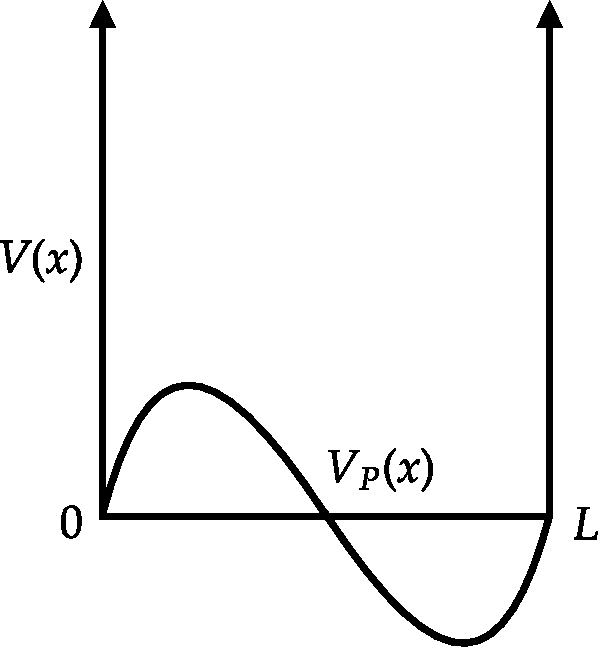
\includegraphics[height=4cm,width=5cm]{gate 2010}
		\end{figure}
	\end{minipage}
	\begin{tasks}(2)
		\task[\textbf{A.}]$E^{(1)}=0 ; E^{(2)}<0$
		\task[\textbf{B.}]$E^{(1)}>0 ; E^{(2)}=0$
		\task[\textbf{C.}]$E^{(1)}=0 ; E^{(2)}$ depends on the sign of $V_{0}$
		\task[\textbf{D.}]$E^{(1)}<0 ; E^{(2)}<0$
	\end{tasks}
	\begin{answer}
		$$E_{1}^{1}=\frac{2}{L} \int_{0}^{L} V_{0} \sin \frac{2 \pi x}{L} d x=0 ; E_{1}^{2}=\sum_{m \neq 1} \frac{\left|\left\langle\psi_{m}\left|V_{P}\right| \psi_{1}\right\rangle\right|^{2}}{E_{1}-E_{m}} \quad \because E_{1}<E_{m} \text { so } E_{1}^{2}=-v e$$
		The correct option is \textbf{(a)}
	\end{answer}
	\begin{minipage}{\textwidth}
		\item The normalized eigenstates of a particle in a one-dimensional potential well
		$$
		V(x)= \begin{cases}0 & \text { if } 0 \leq x \leq a \\ \infty & \text { otherwise }\end{cases}
		$$
		are given by $\psi_{n}(x)=\sqrt{\frac{2}{a}} \sin \left(\frac{n \pi x}{a}\right)$, where $n=1,2,3, \ldots . .$
		The particle is subjected to a perturbation
		$$
		V^{\prime}(x)= \begin{cases}V_{0} \cos \left(\frac{\pi x}{a}\right), & \text { for } 0 \leq x \leq \frac{a}{2} \\ 0, & \text { otherwise }\end{cases}
		$$
		The shift in the ground state energy due to the perturbation, in the first order perturbation theory,
		\exyear{GATE 2011}
	\end{minipage}
	\begin{tasks}(2)
		\task[\textbf{A.}] $\frac{2 V_{o}}{3 \pi}$
		\task[\textbf{B.}]$\frac{V_{o}}{3 \pi}$
		\task[\textbf{C.}]$-\frac{V_{o}}{3 \pi}$
		\task[\textbf{D.}]$-\frac{2 V_{o}}{3 \pi}$
	\end{tasks}
	\begin{answer}
		$$E_{1}^{1}=\int_{0}^{a / 2} \psi_{1}^{*} V^{\prime}(x) \psi_{1} d x=\frac{2}{a} \int_{0}^{a / 2} \sin ^{2}\left(\frac{\pi x}{a}\right) V_{0} \cos \left(\frac{\pi x}{a}\right) d x=\left.\frac{2}{a} V_{0} \frac{\sin ^{3} \frac{\pi x}{a}}{3 \frac{\pi}{a}}\right|_{0} ^{a / 2}=\frac{2 V_{0}}{3 \pi}$$
		The correct option is \textbf{(a)}	
	\end{answer}
	\begin{minipage}{\textwidth}
		\item Consider a system in the unperturbed state described by the Hamiltonian, $H_{0}=\left(\begin{array}{ll}1 & 0 \\ 0 & 1\end{array}\right)$. The system is subjected to a perturbation of the form $H^{\prime}=\left(\begin{array}{ll}\delta & \delta \\ \delta & \delta\end{array}\right)$, where $\delta \ll<1$. The energy eigenvalues of the perturbed system using the first order perturbation approximation are
		\exyear{GATE 2012}
	\end{minipage}
	\begin{tasks}(2)
		\task[\textbf{A.}]1 and $(1+2 \delta)$
		\task[\textbf{B.}]$(1+\delta)$ and $(1-\delta)$
		\task[\textbf{C.}]$(1+2 \delta)$ and $(1-2 \delta)$
		\task[\textbf{D.}]$(1+\delta)$ and $(1-2 \delta)$
	\end{tasks}
	\begin{answer}
		$H_{0}+H^{\prime}, H_{0}$ is degenerate so after using degenerate perturbation through diagonalized $H^{\prime}$ one will get $H^{\prime}=\delta\left(\begin{array}{ll}2 & 0 \\ 0 & 0\end{array}\right), H=\left(\begin{array}{ll}1 & 0 \\ 0 & 1\end{array}\right)+\delta\left(\begin{array}{ll}2 & 0 \\ 0 & 0\end{array}\right)$.
		So $E=1+2 \delta$ and $1+0 \delta$.	\\
		The correct option is \textbf{(a)}
	\end{answer}
	\textbf{\text { Common data questions } 4 \text { and } 5}\\
	$\begin{aligned}
	&\text { To the given unperturbed Hamiltonian }\left[\begin{array}{ccc}
	5 & 2 & 0 \\
	2 & 5 & 0 \\
	0 & 0 & 2
	\end{array}\right] \\
	&\text { we add a small perturbation given by } \varepsilon\left[\begin{array}{ccc}
	1 & 1 & 1 \\
	1 & 1 & -1 \\
	1 & -1 & 1
	\end{array}\right] \text { where } \varepsilon \text { is small quantity. }
	\end{aligned}$\\
	\begin{minipage}{\textwidth}
		\item $\text { The ground state eigenvector of the unperturbed Hamiltonian is }$
		\exyear{GATE 2013}
	\end{minipage}
	\begin{tasks}(2)
		\task[\textbf{A.}] $(1 / \sqrt{2}, 1 \sqrt{2}, 0)$
		\task[\textbf{B.}]$(1 / \sqrt{2},-1 / \sqrt{2}, 0)$
		\task[\textbf{C.}] $(0,0,1)$
		\task[\textbf{D.}]$(1,0,0)$
	\end{tasks}
	\begin{answer}
		$H_{0}=\left[\begin{array}{lll}
		5 & 2 & 0 \\
		2 & 5 & 0 \\
		0 & 0 & 2
		\end{array}\right], H_{P}=\varepsilon\left(\begin{array}{ccc}
		1 & 1 & 1 \\
		1 & 1 & -1 \\
		1 & -1 & 1
		\end{array}\right)$\\
		Eigen value of $H_{0}$ is $E_{1}=2, E_{2}=3, E_{3}=7$ and the Eigen vector corresponds to $\left|\phi_{1}\right\rangle=\left(\begin{array}{l}0 \\ 0 \\ 1\end{array}\right), \quad\left|\phi_{2}\right\rangle=\frac{1}{\sqrt{2}}\left(\begin{array}{c}1 \\ -1 \\ 0\end{array}\right), \quad\left|\phi_{3}\right\rangle=\frac{1}{\sqrt{2}}\left(\begin{array}{l}1 \\ 1 \\ 0\end{array}\right) .$\\
		The correct option is \textbf{(c)}
	\end{answer}
	\begin{minipage}{\textwidth}
		\item A pair of eigenvalues of the perturbed Hamiltonian, using first order perturbation theory, is
		\exyear{GATE 2013}
	\end{minipage}
	\begin{tasks}(2)
		\task[\textbf{A.}]$3+2 \varepsilon, 7+2 \varepsilon$
		\task[\textbf{B.}]$3+2 \varepsilon,+2+\varepsilon$
		\task[\textbf{C.}]$3,7+2 \varepsilon$
		\task[\textbf{D.}]$3,2+2 \varepsilon$
	\end{tasks}
	\begin{answer}
		$E_{1}^{\prime}=\left\langle\phi_{1}\left|H_{P}\right| \phi_{1}\right\rangle=1 \varepsilon \Rightarrow E_{1}=2+1 \varepsilon$
		$$
		\begin{aligned}
		&E_{2}^{\prime}=\left\langle\phi_{2}\left|H_{P}\right| \phi_{2}\right\rangle=\frac{1}{\sqrt{2}}\left(\begin{array}{lll}
		1 & -1 & 0
		\end{array}\right) \cdot \varepsilon\left(\begin{array}{ccc}
		1 & 1 & 1 \\
		1 & 1 & -1 \\
		1 & -1 & 1
		\end{array}\right) \cdot \frac{1}{\sqrt{2}}\left(\begin{array}{c}
		1 \\
		-1 \\
		0
		\end{array}\right)=\epsilon\left(\begin{array}{lll}
		0 & 0 & 1
		\end{array}\right)\left(\begin{array}{c}
		1 \\
		-1 \\
		0
		\end{array}\right)=0 \\
		&E_{3}^{\prime}=\left\langle\phi_{3}\left|H_{P}\right| \phi_{3}\right\rangle=\frac{1}{\sqrt{2}}\left(\begin{array}{lll}
		1 & 1 & 0
		\end{array}\right) \cdot \varepsilon\left(\begin{array}{ccc}
		1 & 1 & 1 \\
		1 & 1 & -1 \\
		1 & -1 & 1
		\end{array}\right) \cdot \frac{1}{\sqrt{2}}\left(\begin{array}{l}
		1 \\
		1 \\
		0
		\end{array}\right)=\varepsilon \cdot \frac{1}{2}\left(\begin{array}{lll}
		2 & 2 & 0
		\end{array}\right) \cdot\left(\begin{array}{l}
		1 \\
		1 \\
		0
		\end{array}\right) \\
		&\Rightarrow E_{3}^{\prime}=\frac{1}{2}(4) \varepsilon=2 \varepsilon \\
		&E_{1}=2+1 \varepsilon, E_{2}=3+0 \varepsilon, E_{3}=7+2 \varepsilon .
		\end{aligned}
		$$
		The correct option is \textbf{(c)}
	\end{answer}
	\begin{minipage}{\textwidth}
		\item A particle is confined to a one dimensional potential box, with the potential
		$$
		V(x)= \begin{cases}0, & 0<x<a \\ \infty, & \text { otherwise }\end{cases}
		$$
		If particle is subjected to a perturbation within the box. $W=\beta x$. Where $\beta$ is small constant, the first order correction to the ground state energy is
		\exyear{GATE 2014}
	\end{minipage}
	\begin{tasks}(2)
		\task[\textbf{A.}] 0
		\task[\textbf{B.}]$a \beta / 4$
		\task[\textbf{C.}]$a \beta / 2$
		\task[\textbf{D.}] $a \beta$
	\end{tasks}
	\begin{answer}
		First order energy correction is $\langle W\rangle=\beta\langle x\rangle$. The average value of position in ground state is $\langle x\rangle=\frac{a}{2} \quad$ so answer is $a \beta / 2$\\
		The correct option is \textbf{(c)}	
	\end{answer}
	\begin{minipage}{\textwidth}
		\item A particle is confined in a box of length $L$ as shown in the figure. If the potential $V_{0}$ is treated as a perturbation, including the first order correction, the ground state energy is
		\exyear{GATE 2015}
		\begin{figure}[H]
			\centering
			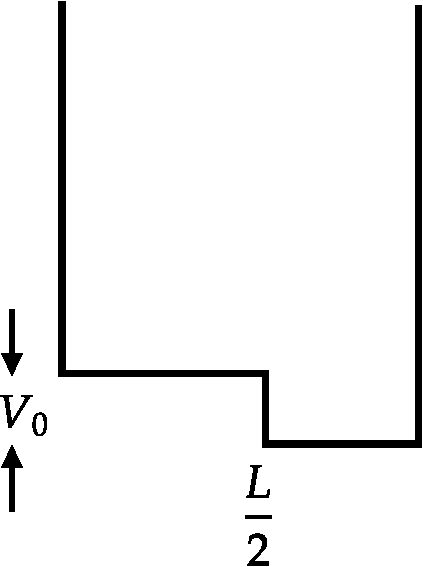
\includegraphics[height=3cm,width=4cm]{diagram-20210824(7)-crop}
		\end{figure}
	\end{minipage}
	\begin{tasks}(2)
		\task[\textbf{A.}] $E=\frac{\hbar^{2} \pi^{2}}{2 m L^{2}}+V_{0}$
		\task[\textbf{B.}]$E=\frac{\hbar^{2} \pi^{2}}{2 m L^{2}}-\frac{V_{0}}{2}$
		\task[\textbf{C.}] $E=\frac{\hbar^{2} \pi^{2}}{2 m L^{2}}+\frac{V_{0}}{4}$
		\task[\textbf{D.}]$E=\frac{\hbar^{2} \pi^{2}}{2 m L^{2}}+\frac{V_{0}}{2}$
	\end{tasks}
	\begin{answer}
		$\begin{aligned}
		&E_{0}^{1}=\frac{2}{L}\left[\int_{0}^{\frac{L}{2}} V_{0} \sin ^{2} \frac{\pi x}{L} d x+\int_{\frac{L}{2}}^{L} 0 \times \sin ^{2} \frac{\pi x}{L} d x\right] \\
		&\Rightarrow E_{0}^{1}=\frac{2}{L} \frac{V_{0}}{2} \int_{0}^{\frac{L}{2}}\left(1-\cos \frac{2 \pi x}{L}\right) d x=\frac{V_{0}}{L}\left[x-\sin \left(\frac{2 \pi x}{L}\right) \frac{L}{2 \pi}\right]_{0}^{\frac{L}{2}} \\
		&\Rightarrow E_{0}^{1}=\frac{V_{0}}{2} \Rightarrow E=\frac{\hbar^{2} \pi^{2}}{2 m L^{2}}+\frac{V_{0}}{2}
		\end{aligned}$
		The correct option is \textbf{(d)}	
	\end{answer}
	\begin{minipage}{\textwidth}
		\item A one dimensional simple harmonic oscillator with Hamiltonian $H_{0}=\frac{p^{2}}{2 m}+\frac{1}{2} k x^{2}$ is subjected to a small perturbation, $H_{1}=\alpha x+\beta x^{3}+\gamma x^{4}$. The first order correction to the ground state energy is dependent on
		\exyear{GATE 2017}
	\end{minipage}
	\begin{tasks}(2)
		\task[\textbf{A.}] only $\beta$
		\task[\textbf{B.}]$\alpha$ and $\gamma$
		\task[\textbf{C.}]$\alpha$ and $\beta$
		\task[\textbf{D.}]only $\gamma$
	\end{tasks}
	\begin{answer}
		$H_{1}=\alpha x+\beta x^{3}+\gamma x^{4}, E_{g}^{1}=\alpha\langle x\rangle+\beta\left\langle x^{3}\right\rangle+\gamma\left\langle x^{4}\right\rangle,\langle x\rangle=0,\left\langle x^{3}\right\rangle=0,\left\langle x^{4}\right\rangle \neq 0$\\
		The correct option is \textbf{(d)}	
	\end{answer}
	
\end{enumerate}